\documentclass[../master/master.tex]{subfiles}

\begin{document}

%----------------------------------------------------------------------
% LECTURE 6: Topic
% Date: February 10, 2026
%----------------------------------------------------------------------
\renewcommand{\lecturenum}{6}
\renewcommand{\lecturedate}{February 10, 2026}
\renewcommand{\lecturetopic}{Connectedness, Continuity, Uniform Continuity}

\section{Lecture \lecturenum : \lecturedate}

\begin{lecturesummary}
\textbf{Lecture Overview:} We begin with the definitions of separated and connected sets, and characterize connected subsets of $\R$ as those with no gaps. We then define continuity (via preimages of open sets, bases, locality, and $\eps$-$\delta$), homeomorphisms, and prove that continuous functions preserve compactness and connectedness. From these we derive the extreme value theorem, the intermediate value theorem, and that continuous functions on compact sets are uniformly continuous.
\end{lecturesummary}

\subsection{Separated and Connected Sets}

\begin{summarybox}
\textbf{Section Overview:} We define separated sets and connected sets. A subset $E \subset \R$ is connected if and only if it has no ``gaps'' --- whenever $x, y \in E$ and $x < z < y$, then $z \in E$. We prove this characterization in both directions.
\end{summarybox}

\begin{definition}
Two subsets $A, B \subset X$ are \defn{separated} if $\overline{A} \cap B = \emptyset$ and $A \cap \overline{B} = \emptyset$.
\end{definition}

\begin{definition}
A set $E \subset X$ is \defn{connected} if $E$ is \emph{not} a union $A \cup B$ where $A$ and $B$ are nonempty and separated.
\end{definition}

\begin{example}
Consider the sets $A = (1, 2)$ and $B = (3, 4)$ in $\R$.

\begin{center}
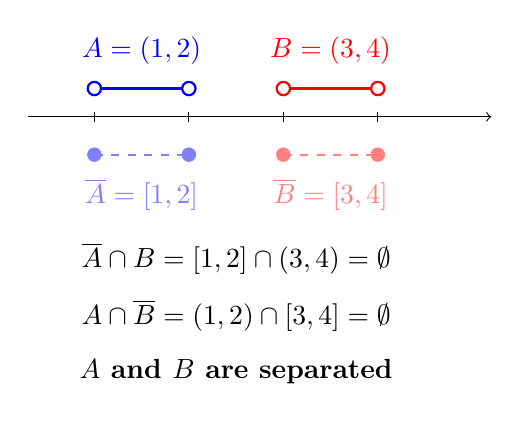
\begin{tikzpicture}[scale=1.2]
  % Number line
  \draw[->] (0.3,0) -- (5.2,0);

  % Set A (open interval)
  \draw[thick, blue] (1,0.3) -- (2,0.3);
  \filldraw[white, draw=blue, thick] (1,0.3) circle (2pt);
  \filldraw[white, draw=blue, thick] (2,0.3) circle (2pt);
  \node[blue, above] at (1.5, 0.45) {$A = (1,2)$};

  % Closure of A (dashed)
  \draw[dashed, blue!50, thick] (1,-0.4) -- (2,-0.4);
  \filldraw[blue!50] (1,-0.4) circle (2pt);
  \filldraw[blue!50] (2,-0.4) circle (2pt);
  \node[blue!50, below] at (1.5, -0.55) {$\overline{A} = [1,2]$};

  % Set B (open interval)
  \draw[thick, red] (3,0.3) -- (4,0.3);
  \filldraw[white, draw=red, thick] (3,0.3) circle (2pt);
  \filldraw[white, draw=red, thick] (4,0.3) circle (2pt);
  \node[red, above] at (3.5, 0.45) {$B = (3,4)$};

  % Closure of B (dashed)
  \draw[dashed, red!50, thick] (3,-0.4) -- (4,-0.4);
  \filldraw[red!50] (3,-0.4) circle (2pt);
  \filldraw[red!50] (4,-0.4) circle (2pt);
  \node[red!50, below] at (3.5, -0.55) {$\overline{B} = [3,4]$};

  % Tick marks
  \foreach \x in {1, 2, 3, 4} {
    \draw (\x, -0.05) -- (\x, 0.05);
  }

  % Annotation
  \node[align=center] at (2.5, -1.5) {$\overline{A} \cap B = [1,2] \cap (3,4) = \emptyset$};
  \node[align=center] at (2.5, -2.1) {$A \cap \overline{B} = (1,2) \cap [3,4] = \emptyset$};
  \node[align=center, font=\bfseries] at (2.5, -2.7) {$A$ and $B$ are separated};
\end{tikzpicture}
\end{center}
\end{example}

\begin{theorem}
$E \subset \R$ is connected if and only if for all $x, y \in E$ and for all $z$ with $x < z < y$, we have $z \in E$.
\end{theorem}

\begin{proof}
$(\Rightarrow)$ Suppose $E$ is connected. We proceed by contradiction. Assume there exist $x, y \in E$ and $z$ with $x < z < y$ but $z \notin E$. Let
\[
A = E \cap (-\infty, z), \qquad B = E \cap (z, \infty).
\]
Then $A$ is nonempty (since $x \in A$) and $B$ is nonempty (since $y \in B$). Since $z \notin E$, we have $A \cup B = E$. Moreover, $\overline{A} \subset (-\infty, z]$ and $\overline{B} \subset [z, \infty)$, so
\[
\overline{A} \cap B = \emptyset \quad \text{and} \quad A \cap \overline{B} = \emptyset.
\]
Thus $A$ and $B$ are nonempty, separated, and $E = A \cup B$, contradicting the assumption that $E$ is connected.

$(\Leftarrow)$ We prove the contrapositive. Suppose $E$ is not connected, so $E = A \cup B$ where $A, B$ are nonempty and separated. Pick $x \in A$, $y \in B$; without loss of generality assume $x < y$. Let
\[
z = \sup(A \cap [x, y]).
\]
This exists since $A \cap [x, y]$ is nonempty (contains $x$) and bounded above by $y$.

Since $z = \sup(A \cap [x, y])$, we have $z \in \overline{A}$. Since $\overline{A} \cap B = \emptyset$, we get $z \notin B$. Since $y \in B$ and $z \notin B$, we have $z \neq y$, so $z < y$.

\textbf{Case 1:} $z \notin A$. Then $z \notin A \cup B = E$, but $x, y \in E$ and $x \leq z < y$. If $z = x$ then $z = x \in A$, a contradiction, so $x < z < y$ and $z \notin E$.

\textbf{Case 2:} $z \in A$. Then since $A \cap \overline{B} = \emptyset$, we have $z \notin \overline{B}$, so there exists $\eps > 0$ such that $(z - \eps, z + \eps) \cap B = \emptyset$. Choose $\eps$ small enough so that $z + \eps < y$. Since $z = \sup(A \cap [x, y])$, no element of $A$ lies in $(z, z + \eps)$. So any point $z' \in (z, z + \eps)$ satisfies $z' \notin A$ and $z' \notin B$, hence $z' \notin E$. But $x < z' < y$ with $x, y \in E$.

In both cases, we find a point strictly between two elements of $E$ that is not in $E$.
\end{proof}

\subsection{Continuous Functions}

\begin{summarybox}
\textbf{Section Overview:} We define continuity via preimages of open sets and give three equivalent formulations: via a basis, locally, and via $\eps$-$\delta$. We show that sums, compositions, and quotients of continuous functions are continuous, and define homeomorphisms.
\end{summarybox}

\begin{remark}
Connectedness and compactness are described purely in set-theoretic terms. From them, we obtain topological properties.
\end{remark}

\begin{definition}
A function $f : X \to Y$ is \defn{continuous} if for all $V$ open in $Y$, $f^{-1}(V)$ is open in $X$.

Properties of continuous functions:
\begin{enumerate}
  \item \textbf{Basis:} Given a basis $\mathcal{B}$ of $Y$, to check that $f$ is continuous it suffices to check that $f^{-1}(B)$ is open in $X$ for all $B \in \mathcal{B}$.
  \item \textbf{Locality:} $f$ is \defn{continuous at $\alpha$} if there exists an open neighborhood $U_\alpha$ of $\alpha$ such that $f|_{U_\alpha}$ is continuous.
  \item \textbf{$\eps$-$\delta$ (open balls):} In $\R^n$, $f$ is continuous at $x$ if for all $\eps > 0$ there exists $\delta > 0$ such that
  \[
  |x - y| < \delta \implies |f(y) - f(x)| < \eps.
  \]
\end{enumerate}
\end{definition}

\begin{example}
$f : (-1, 1) \to \R$ defined by $f(x) = \dfrac{x}{1 - x^2}$.

This mapping is one-to-one. Its inverse is $f^{-1}(y) = \dfrac{2y}{1 + \sqrt{1 + 4y^2}}$.

\begin{center}
\begin{tikzpicture}[scale=0.9]
  % --- Left plot: f ---
  % Axes
  \draw[->] (-2.5, 0) -- (2.5, 0) node[right] {$x$};
  \draw[->] (0, -2.2) -- (0, 2.2) node[above] {$y$};

  % Asymptotes
  \draw[dashed, gray] (-1, -2.2) -- (-1, 2.2) node[above, gray] {\small $-1$};
  \draw[dashed, gray] (1, -2.2) -- (1, 2.2) node[above, gray] {\small $1$};

  % Function f(x) = x/(1-x^2) on (-1, 1), clipped
  \begin{scope}
    \clip (-1.5, -2.2) rectangle (1.5, 2.2);
    \draw[thick, blue, domain=-0.95:0.95, samples=200] plot (\x, {\x/(1-\x*\x)});
  \end{scope}

  % Label
  \node[blue] at (0, -2.8) {$f(x) = \dfrac{x}{1-x^2}$};

  % --- Right plot: f^{-1} ---
  \begin{scope}[xshift=7.5cm]
    % Axes
    \draw[->] (-3.5, 0) -- (3.5, 0) node[right] {$y$};
    \draw[->] (0, -2.2) -- (0, 2.2) node[above] {$x$};

    % Asymptotes
    \draw[dashed, gray] (-3.5, 1) -- (3.5, 1) node[right, gray] {\small $1$};
    \draw[dashed, gray] (-3.5, -1) -- (3.5, -1) node[right, gray] {\small $-1$};

    % Function f^{-1}(y) = 2y / (1 + sqrt(1+4y^2))
    \draw[thick, red, domain=-3.3:3.3, samples=200] plot (\x, {2*\x/(1+sqrt(1+4*\x*\x))});

    % Label
    \node[red] at (0, -2.8) {$f^{-1}(y) = \dfrac{2y}{1 + \sqrt{1+4y^2}}$};
  \end{scope}
\end{tikzpicture}
\end{center}
\end{example}

Consider the projection mappings $\pi_i : \R^n \to \R$ defined by $(x_1, \ldots, x_n) \mapsto x_i$.

\begin{theorem}
If $f, g : X \to \R$ are continuous, then:
\begin{enumerate}
  \item $f + g$ is continuous,
  \item $f \circ g$ is continuous,
  \item $f/g$ is continuous (wherever $g \neq 0$).
\end{enumerate}
\end{theorem}

% TODO: fill in eps-delta proofs for f+g, fg

\begin{definition}
If $f : X \to Y$ is a bijection and both $f$ and $f^{-1}$ are continuous, then $f$ is a \defn{homeomorphism}. We write $X \sim Y$.
\end{definition}

\subsection{Topology of Continuous Functions}

\begin{summarybox}
\textbf{Section Overview:} Continuous functions preserve key topological properties: compact sets map to compact sets, and connected sets map to connected sets. As a consequence, continuous functions on compact sets attain their maximum and minimum.
\end{summarybox}

\begin{theorem}
Continuous functions preserve compactness and connectedness. If $E \subset X$ is compact (resp.\ connected) and $f : X \to Y$ is continuous, then $f(E)$ is compact (resp.\ connected).
\end{theorem}

\begin{notebox}
Take the interval $E = [0, 1] \subset \R$. Since $E$ is compact, $f(E)$ is compact, hence closed and bounded (by Heine--Borel). In particular, $f$ attains its maximum and minimum on $E$.
\end{notebox}

\begin{proof}[Proof (compactness)]
Let $\{V_\alpha\}$ be an open cover of $f(K)$. Since $f$ is continuous, each $f^{-1}(V_\alpha)$ is open in $X$. The collection $\{f^{-1}(V_\alpha)\}$ is an open cover of $K$. Since $K$ is compact, there exist finitely many indices $\alpha_1, \ldots, \alpha_n$ such that
\[
K \subset f^{-1}(V_{\alpha_1}) \cup \cdots \cup f^{-1}(V_{\alpha_n}).
\]
Applying $f$ to both sides,
\[
f(K) \subset V_{\alpha_1} \cup \cdots \cup V_{\alpha_n}.
\]
Thus $\{V_{\alpha_1}, \ldots, V_{\alpha_n}\}$ is a finite subcover of $f(K)$.
\end{proof}

\begin{proof}[Proof (connectedness)]
Suppose for contradiction that $f(E)$ is not connected. Then $f(E) = A \cup B$ where $A, B$ are nonempty and separated. Let $G = E \cap f^{-1}(A)$ and $H = E \cap f^{-1}(B)$. Then $G$ and $H$ are nonempty (since $A$ and $B$ are nonempty subsets of $f(E)$) and $G \cup H = E$ (since every point of $E$ maps into $A$ or $B$).

We claim $G$ and $H$ are separated. Since $A$ and $B$ are separated, $\overline{A} \cap B = \emptyset$. If $p \in \overline{G} \cap H$, then $f(p) \in B$. Since $f$ is continuous and $p$ is a limit point of $G$ (or in $G$), we have $f(p) \in \overline{f(G)} \subset \overline{A}$. But then $f(p) \in \overline{A} \cap B = \emptyset$, a contradiction. Thus $\overline{G} \cap H = \emptyset$. By symmetry, $G \cap \overline{H} = \emptyset$.

So $E = G \cup H$ with $G, H$ nonempty and separated, contradicting the connectedness of $E$.
\end{proof}

\begin{theorem}
Let $f$ be a continuous function on a compact set $K$. Define $M = \sup_{x \in K} f(x)$ and $m = \inf_{x \in K} f(x)$. Then there exist $p, q \in K$ such that $f(p) = M$ and $f(q) = m$.
\end{theorem}

\begin{proof}
Since $K$ is compact and $f$ is continuous, $f(K)$ is compact (by the previous theorem), hence closed and bounded by Heine--Borel. Since $f(K)$ is bounded, $M = \sup f(K)$ and $m = \inf f(K)$ are finite. Since $f(K)$ is closed, it contains all its limit points. But $M = \sup f(K)$ is a limit point of $f(K)$ (for every $\eps > 0$, there exists $y \in f(K)$ with $M - \eps < y \leq M$), so $M \in f(K)$. Thus there exists $p \in K$ with $f(p) = M$. Similarly, $m \in f(K)$, so there exists $q \in K$ with $f(q) = m$.
\end{proof}

\begin{theorem}[Intermediate Value Theorem]
If $f$ is continuous on $[a, b]$ and $f(a) < c < f(b)$, then there exists $p \in (a, b)$ such that $f(p) = c$.
\end{theorem}

\begin{proof}
Since $f$ is continuous and $[a, b]$ is connected, $f([a, b])$ is connected (by the connectedness theorem above). Since $f([a, b]) \subset \R$ is connected, it has no gaps: for any two values in $f([a, b])$ and anything between them, that value is also in $f([a, b])$. We have $f(a), f(b) \in f([a, b])$ and $f(a) < c < f(b)$, so $c \in f([a, b])$. Thus there exists $p \in [a, b]$ with $f(p) = c$. Since $f(a) < c < f(b)$, we have $f(p) \neq f(a)$ and $f(p) \neq f(b)$, so $p \neq a$ and $p \neq b$, hence $p \in (a, b)$.
\end{proof}

\begin{definition}
A function $f : X \to Y$ is \defn{uniformly continuous} if for all $\eps > 0$ there exists $\delta > 0$ such that for all $p, q \in X$,
\[
d_X(p, q) < \delta \implies d_Y(f(p), f(q)) < \eps.
\]
\end{definition}

\begin{theorem}
If $K$ is compact and $f : K \to Y$ is continuous, then $f$ is uniformly continuous.
\end{theorem}

\begin{proof}
Let $\eps > 0$. Since $f$ is continuous, for each $p \in K$ there exists $\delta_p > 0$ such that
\[
d_X(x, p) < \delta_p \implies d_Y(f(x), f(p)) < \frac{\eps}{2}.
\]
The collection $\{B(p, \delta_p / 2) : p \in K\}$ is an open cover of $K$. Since $K$ is compact, there exist finitely many $p_1, \ldots, p_n \in K$ such that
\[
K \subset B(p_1, \delta_{p_1}/2) \cup \cdots \cup B(p_n, \delta_{p_n}/2).
\]
Let $\delta = \frac{1}{2} \min(\delta_{p_1}, \ldots, \delta_{p_n}) > 0$. Now suppose $p, q \in K$ with $d_X(p, q) < \delta$. Since the balls cover $K$, there exists $p_i$ with $p \in B(p_i, \delta_{p_i}/2)$, i.e.\ $d_X(p, p_i) < \delta_{p_i}/2$. Then
\[
d_X(q, p_i) \leq d_X(q, p) + d_X(p, p_i) < \delta + \frac{\delta_{p_i}}{2} \leq \frac{\delta_{p_i}}{2} + \frac{\delta_{p_i}}{2} = \delta_{p_i}.
\]
So $d_Y(f(p), f(p_i)) < \eps/2$ and $d_Y(f(q), f(p_i)) < \eps/2$, and by the triangle inequality,
\[
d_Y(f(p), f(q)) \leq d_Y(f(p), f(p_i)) + d_Y(f(p_i), f(q)) < \frac{\eps}{2} + \frac{\eps}{2} = \eps. \qedhere
\]
\end{proof}

\begin{theorem}
Let $E \subset \R$ be a non-compact set. Then there exists a continuous function on $E$ that is:
\begin{enumerate}
  \item not bounded,
  \item bounded but does not attain its maximum,
  \item not uniformly continuous.
\end{enumerate}
\end{theorem}

\begin{proof}
Since $E$ is not compact, by Heine--Borel $E$ is either not closed or not bounded.

\textbf{Case 1: $E$ is not bounded.} Then $f(x) = x$ is continuous on $E$ and not bounded. The function $g(x) = \dfrac{x^2}{1 + x^2}$ is continuous and bounded with $0 \leq g < 1$, but $\sup g = 1$ is never attained. The function $h(x) = x^2$ is continuous but not uniformly continuous (for any $\delta > 0$, choose $x$ large enough so that $|x^2 - (x + \delta/2)^2| > 1$).

\textbf{Case 2: $E$ is bounded but not closed.} Then there exists a limit point $x_0$ of $E$ with $x_0 \notin E$. Define $f(x) = \dfrac{1}{x - x_0}$, which is continuous on $E$ but not bounded. The function $g(x) = \dfrac{1}{1 + (x - x_0)^{-2}}$ is continuous and bounded with $0 < g < 1$, but $\sup g = 1$ is never attained (it would require $|x - x_0| \to \infty$, but $E$ is bounded). The function $h(x) = \dfrac{1}{x - x_0}$ is not uniformly continuous (as $x \to x_0$, arbitrarily close points have arbitrarily far images).
\end{proof}

\end{document}
